%%%%%%%%%%%%%%%%%%%%%%%%%%%%%%%%%%%%%%%%%%%%%%%%%%%%%%%%%%%%%%%%%%%%%%%%%%%%%%%%%
\section{Introduction}
%%%%%%%%%%%%%%%%%%%%%%%%%%%%%%%%%%%%%%%%%%%%%%%%%%%%%%%%%%%%%%%%%%%%%%%%%%%%%%%%%
\subsection{Scalar Model}
%%%%%%%%%%%%%%%%%%%%%%%%%%%%%%%%%%%%%%%%%%%%%%%%%%%%%%%%%%%%%%%%%%%%%%%%%%%%%%%%%
\begin{frame}
\frametitle{Radiation Transport}

\begin{itemize}
  \item Consider the following model for radiation transport:
    \begin{equation}\label{eq:rad_transport}
      \frac{1}{\speed}\ppt{\angularflux}
        + \directionvector\cdot\nabla\angularflux(\x,\directionvector,E,t)
        + \totalcrosssection(\x,E)\angularflux(\x,\directionvector,E,t)
        = \radiationsource(\x,\directionvector,E,t) \eqp
    \end{equation}
  \item For example, $\radiationsource\xt$ can include extraneous sources
    and scattering sources in a source iteration scheme:
    \begin{equation}
      \frac{1}{\speed}\ppt{\angularflux_d}^{(\ell+1)}
        + \directionvector_d\cdot\nabla\angularflux_d^{(\ell+1)}
        + \totalcrosssection(\x)\angularflux_d^{(\ell+1)}
        = \radiationsource_d^{(\ell)} \eqc
    \end{equation}
    with for example, $\radiationsource_d^{(\ell)}=
    \frac{Q_{ext}}{4\pi} + \frac{\Sigma_s}{4\pi}\scalarflux^{(\ell)}$.
%  \item Consider a more general case of a scalar conservation law:
%    \begin{equation}
%      \pd{\scalarsolution}{t} + \nabla\cdot\consflux(\scalarsolution)
%      + \reactioncoef(\x)\scalarsolution\xt
%      = \scalarsource\xt \eqp
%    \end{equation}
%  \item Radiation transport fits this model with the following substitutions:
%\[
%  \scalarsolution\rightarrow\angularflux
%  \eqc \quad
%  \consflux(\angularflux)\rightarrow\speed\directionvector\angularflux
%  \eqc \quad
%  \reactioncoef\rightarrow\speed\totalcrosssection
%  \eqc \quad
%  \scalarsource\rightarrow\speed\radiationsource
%  \eqp
%\]
\end{itemize}

\end{frame}
%%%%%%%%%%%%%%%%%%%%%%%%%%%%%%%%%%%%%%%%%%%%%%%%%%%%%%%%%%%%%%%%%%%%%%%%%%%%%%%%%
\begin{frame}
\frametitle{Scalar Conservation Law Model}

\begin{itemize}
  \item This research considers the following scalar conservation law model:
    \begin{equation}
      \pd{\scalarsolution}{t} + \nabla\cdot\consflux(\scalarsolution)
      + \textcolor{secondarycolorheavy}{\reactioncoef(\x)\scalarsolution\xt}
      = \textcolor{secondarycolorheavy}{\scalarsource\xt} \eqc
    \end{equation}
    where $\reactioncoef(\x)\ge 0$ and $\scalarsource\xt\ge 0$.
  \item Some examples of applicability include
\begin{tabular}{p{2.5in} c}
  \textcolor{secondarycolorheavy}{Linear advection}:
    advection of some quantity, such as a tracer
    & $\consflux(\scalarsolution)=\velocity\scalarsolution$\\
  %\textcolor{secondarycolorheavy}{1-D Traffic flow}:
  %  vehicle density on a one-lane highway
  %  & $\consfluxletter(\scalarsolution)=
  %    \scalarsolution v_{max}\pr{1-\frac{\scalarsolution}{\scalarsolution_{max}}}$\\
    \textcolor{secondarycolorheavy}{Inviscid Burgers' equation}:
      inviscid fluid flow model capturing some key features of gas dynamics
    & $\consflux(\scalarsolution)=\frac{1}{2}\scalarsolution^2\mathbf{1}$\\
    \textcolor{secondarycolorheavy}{Radiation transport}:
      transport of radiation such as photons or neutrons
    & $\consflux(\scalarsolution)=\speed\di\scalarsolution$
\end{tabular}
%    \begin{itemize}
%      \item \textcolor{secondarycolorheavy}{Linear advection}:
%        advection of some quantity, such as a tracer:
%        $\consflux(\scalarsolution)=\velocity\scalarsolution$
%      \item \textcolor{secondarycolorheavy}{1-D Traffic flow}:
%        vehicle density on a one-lane highway:
%        $\consfluxletter(\scalarsolution)=
%          \scalarsolution v_{max}\pr{1-\scalarsolution/\scalarsolution_{max}}$
%      \item \textcolor{secondarycolorheavy}{Inviscid Burgers' equation}:
%        inviscid fluid flow model capturing some key features of gas dynamics:\\
%        $\consflux(\scalarsolution)=\frac{1}{2}\scalarsolution^2\mathbf{1}$
%      \item \textcolor{secondarycolorheavy}{Radiation transport}:
%        transport of radiation such as photons or neutrons:
%        $\consflux(\scalarsolution)=\speed\di\scalarsolution$
%    \end{itemize}
\end{itemize}

\end{frame}
%%%%%%%%%%%%%%%%%%%%%%%%%%%%%%%%%%%%%%%%%%%%%%%%%%%%%%%%%%%%%%%%%%%%%%%%%%%%%%%%%
\subsection{Shallow Water Equations}
%%%%%%%%%%%%%%%%%%%%%%%%%%%%%%%%%%%%%%%%%%%%%%%%%%%%%%%%%%%%%%%%%%%%%%%%%%%%%%%%%
\begin{frame}
\frametitle{Shallow Water Equations (SWE)}

\begin{itemize}
  \item The shallow water equations are
    \begin{equation}
      \ppt{}\left[\begin{array}{c}\height\\\heightmomentum\end{array}\right]
        + \divergence\left[\begin{array}{c}\heightmomentum\\
          \heightmomentum\otimes\velocity + \half\gravity\height^2 \mathbb{I}
          \end{array}\right]
        = \left[\begin{array}{c}0\\-\gravity\height\nabla\bathymetry\end{array}
    \right] \eqp
    \end{equation}
    \begin{itemize}
      \item $\height\xt \equiv \int\density\xt dz$ is referred to as ``height''.
      \item $\heightmomentum\xt \equiv \height\xt\velocity\xt$ is referred to
        as ``discharge''.
      \item $\gravity$ is the acceleration due to gravity.
      \item $\bathymetry(\x)$ is the bottom topography profile,
        or ``bathymetry''.
    \end{itemize}
  \item Obtained by depth-integrating Navier-Stokes equations with the
    assumption that the horizontal length scale is much greater than the
    vertical length scale
  \item Some important simulations include
    \begin{itemize}
      \item \textcolor{secondarycolorheavy}{dam break problems}: for example, what wave
        structures will develop in a dam-break accident?
      \item \textcolor{secondarycolorheavy}{wave/tsunami problems}: for example, what height
        of seawall is necessary to stop a wave of a certain height?
    \end{itemize}
\end{itemize}

\end{frame}
%%%%%%%%%%%%%%%%%%%%%%%%%%%%%%%%%%%%%%%%%%%%%%%%%%%%%%%%%%%%%%%%%%%%%%%%%%%%%%%%%
\subsection{Conservation Laws}
%%%%%%%%%%%%%%%%%%%%%%%%%%%%%%%%%%%%%%%%%%%%%%%%%%%%%%%%%%%%%%%%%%%%%%%%%%%%%%%%%
\begin{frame}
\frametitle{Modeling Conservation Laws}

\begin{itemize}
  \item The strong form of a conservation law PDE
    \begin{equation}
      \scalarsolution_t + \consfluxletter(\scalarsolution)_x
      = 0
    \end{equation}
    does not hold for discontinuous solutions, so an integral, or \hlorange{weak} form
    is used:
    \begin{equation}
      \int\scalarsolution_t\phi dx
        + \int\consfluxletter(\scalarsolution)_x\phi dx
      = 0 \eqp
    \end{equation}
  \item The solution to the weak problem is not necessarily unique.
    \begin{itemize}
      \item Some physics have been neglected in the hyperbolic PDE model.
      \item In particular, hyperbolic PDEs ignore diffusive/viscous effects.
    \end{itemize}
  \item The physically correct solution is the \hlorange{vanishing viscosity}
    solution, where one takes the limit as $\epsilon\rightarrow0$:
    \begin{equation}
      \scalarsolution^\epsilon_t
        + \consfluxletter(\scalarsolution^\epsilon)_x
      = \epsilon\scalarsolution_{xx}^\epsilon \eqp
    \end{equation}
\end{itemize}

\end{frame}
%%%%%%%%%%%%%%%%%%%%%%%%%%%%%%%%%%%%%%%%%%%%%%%%%%%%%%%%%%%%%%%%%%%%%%%%%%%%%%%%%
\begin{frame}
\frametitle{A Simple Motivating Example}
\framesubtitle{Linear Advection of Discontinuous Wave Front}

\begin{center}
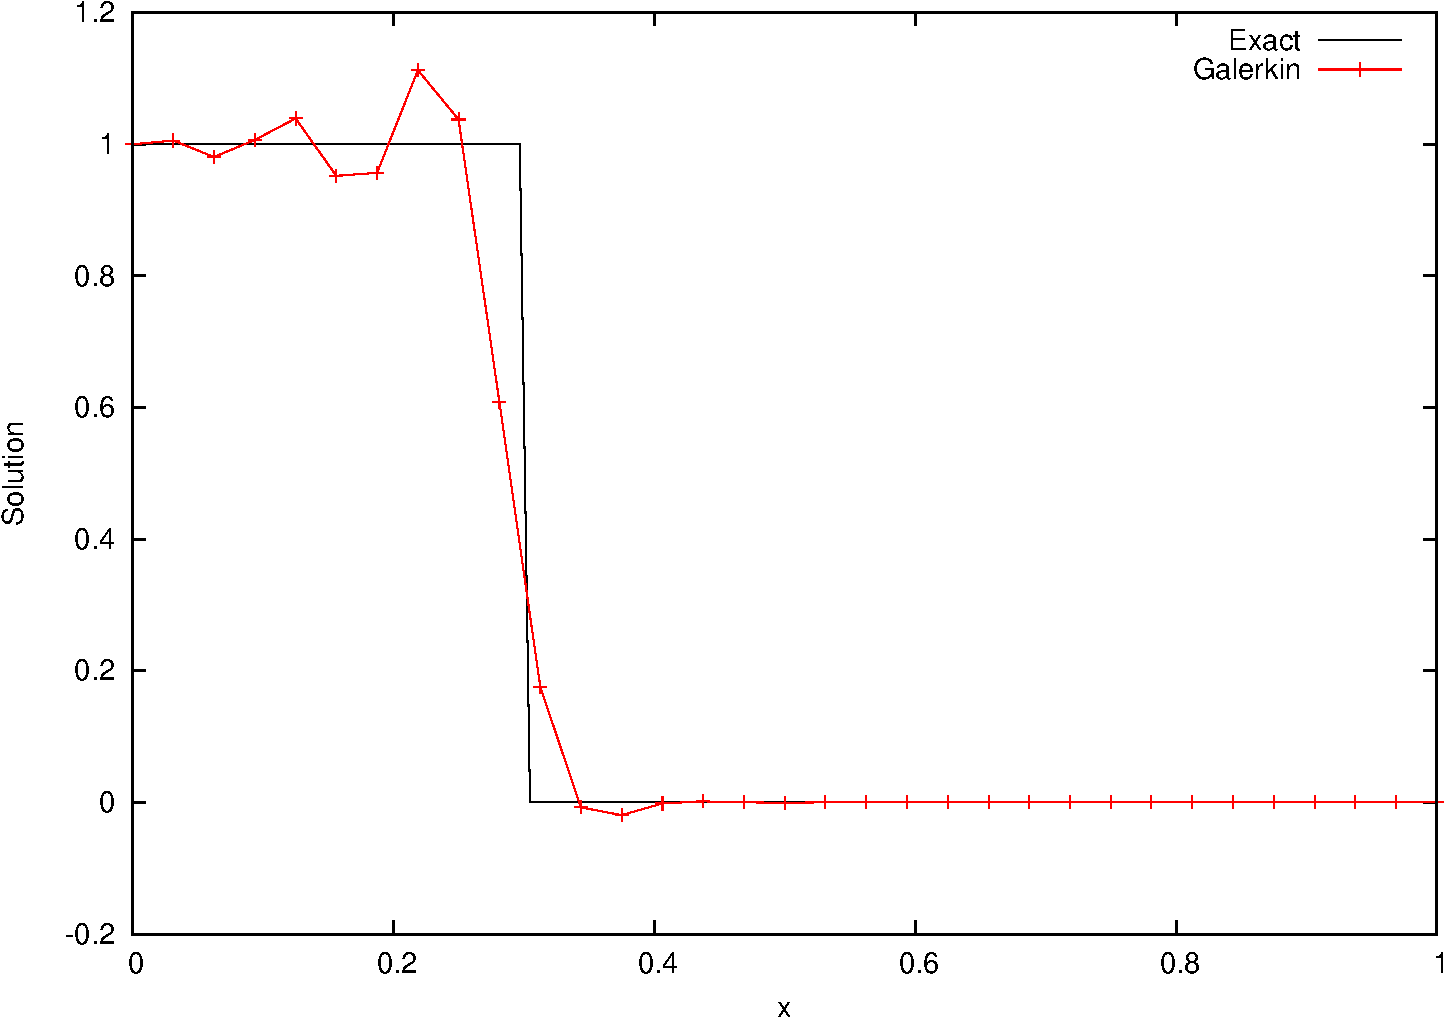
\includegraphics[width=0.85\textwidth]{./figures/advection_Galerkin.pdf}
\end{center}

\end{frame}
%%%%%%%%%%%%%%%%%%%%%%%%%%%%%%%%%%%%%%%%%%%%%%%%%%%%%%%%%%%%%%%%%%%%%%%%%%%%%%%%%
\subsection{Objectives}
%%%%%%%%%%%%%%%%%%%%%%%%%%%%%%%%%%%%%%%%%%%%%%%%%%%%%%%%%%%%%%%%%%%%%%%%%%%%%%%%%
\begin{frame}
\frametitle{Objectives}

\begin{itemize}
   \item The objectives of this research are the following:
   \begin{itemize}
      \item \textcolor{secondarycolorheavy}{Accurately solve conservation law
        problems} using the continuous finite element method (CFEM):
      \begin{itemize}
        \item 2nd-order-accuracy in space (for smooth problems)
        \item convergence to the entropy solution
      \end{itemize}
      \item \textcolor{secondarycolorheavy}{Prevent spurious oscillations}.
      \begin{itemize}
	\item Complete immunity to spurious oscillations remains unattainable for
          high-order schemes, but quality results are possible in practice.
      \end{itemize}
      \item \textcolor{secondarycolorheavy}{Prevent solution from leaving
        physically-motivated bounds}.
      \item \textcolor{secondarycolorheavy}{Prevent negativities}
        for physically non-negative quantities.
   \end{itemize}
\end{itemize}

\end{frame}
%%%%%%%%%%%%%%%%%%%%%%%%%%%%%%%%%%%%%%%%%%%%%%%%%%%%%%%%%%%%%%%%%%%%%%%%%%%%%%%%%
\subsection{Entropy Viscosity}
%%%%%%%%%%%%%%%%%%%%%%%%%%%%%%%%%%%%%%%%%%%%%%%%%%%%%%%%%%%%%%%%%%%%%%%%%%%%%%%%%
\begin{frame}
\frametitle{Entropy Viscosity Method}

\begin{itemize}
  \item Additional conditions/physics are required to filter out
    spurious weak solutions to obtain the physically correct solution.
    \begin{itemize}
      \item Gas dynamics has the second law of thermodynamics
        $\rightarrow$ entropy conditions.
      \item Other PDE systems frequently have similar conditions.
    \end{itemize}
  \item Scalar conservation law \hlorange{entropy condition}:
    \begin{equation}
      \entropy(u)_t + \psi(u)_x \leq 0 \eqc
    \end{equation}
    for all convex entropy $\entropy(u)$ and corresponding flux $\psi(u)$.
  \item The idea of the \hlorange{entropy viscosity} method is to enforce
    the entropy condition with dissipation proportional to the violation
    of the condition.
\end{itemize}

\end{frame}
%%%%%%%%%%%%%%%%%%%%%%%%%%%%%%%%%%%%%%%%%%%%%%%%%%%%%%%%%%%%%%%%%%%%%%%%%%%%%%%%%
\subsection{FCT}
%%%%%%%%%%%%%%%%%%%%%%%%%%%%%%%%%%%%%%%%%%%%%%%%%%%%%%%%%%%%%%%%%%%%%%%%%%%%%%%%%
\begin{frame}
\frametitle{Flux-Corrected Transport (FCT)}

\begin{itemize}
   \item FCT initially developed in 1973 for finite difference methods
      and was more recently applied to CFEM.
   \item FCT mixes
     \begin{itemize}
       \item a \hlorange{high-order scheme}, which may have spurious
         oscillations and negativities, and
       \item a \hlorange{low-order scheme}, which has the desired properties
         such as monotonicity preservation and positivity preservation.
     \end{itemize}
   \item \hlorange{The FCT idea}: Reverse as much artificial diffusion in the
     low-order scheme as possible without producing an unphysical solution.
   \item Summary of the FCT algorithm:
     \begin{enumerate}
       \item Derive \hlorange{antidiffusion source} from low-order scheme to high-order
         scheme.
       \item Decompose antidiffusion source into \hlorange{antidiffusive fluxes} between nodes.
       \item Define physically-motivated \hlorange{solution bounds}:
         \begin{equation}
           u^{min}_i \leq u_i \leq u^{max}_i \quad \forall i \eqp
         \end{equation}
       \item Apply a \hlorange{limiter} to the antidiffusive fluxes to ensure
         that solution bounds are not violated.
     \end{enumerate}
\end{itemize}

\end{frame}
%%%%%%%%%%%%%%%%%%%%%%%%%%%%%%%%%%%%%%%%%%%%%%%%%%%%%%%%%%%%%%%%%%%%%%%%%%%%%%%%%
\subsection{Outline}
%%%%%%%%%%%%%%%%%%%%%%%%%%%%%%%%%%%%%%%%%%%%%%%%%%%%%%%%%%%%%%%%%%%%%%%%%%%%%%%%%
\begin{frame}
\frametitle{Outline}

\begin{itemize}
   \item The scalar case
   \begin{itemize}
      \item Problem formulation
      \item Discretization
      \item Low-order, DMP-satisfying, positivity-preserving scheme
      \item High-order, entropy-based scheme
      \item High-order, DMP-satisfying, positivity-preserving FCT scheme
      \item Scalar results
   \end{itemize}
   \item The systems case (using the shallow water equations)
   \begin{itemize}
      \item Problem formulation
      \item Discretization
      \item Low-order, domain-invariant, positivity-preserving scheme
      \item High-order, entropy-based scheme
      \item High-order, positivity-preserving FCT scheme
      \item Shallow water equations results
   \end{itemize}
   \item Conclusions
\end{itemize}

\end{frame}
